\documentclass{beamer}
\usetheme{metropolis}

\usepackage{array}
\usepackage{caption}
\usepackage{graphicx}
\usepackage{xcolor}

\usepackage{pgfpages}

\setbeameroption{show notes on second screen=right} % Both

\usepackage{pdfpages}

\usepackage[sort&compress]{natbib}
\bibliographystyle{apalike}

\newcommand{\slidenote}[1]{\note[item]{#1}}


\title{Communication in Multi-agent Reinforcement Learning}
\date{\today}
\author{Jack Montgomery}
\institute{MAM4001W: Advanced Topics in Reinforcement Learning}

\begin{document}

\maketitle

\section{Motivation}
\begin{frame}{Motivation}
\begin{figure}
	\centering
	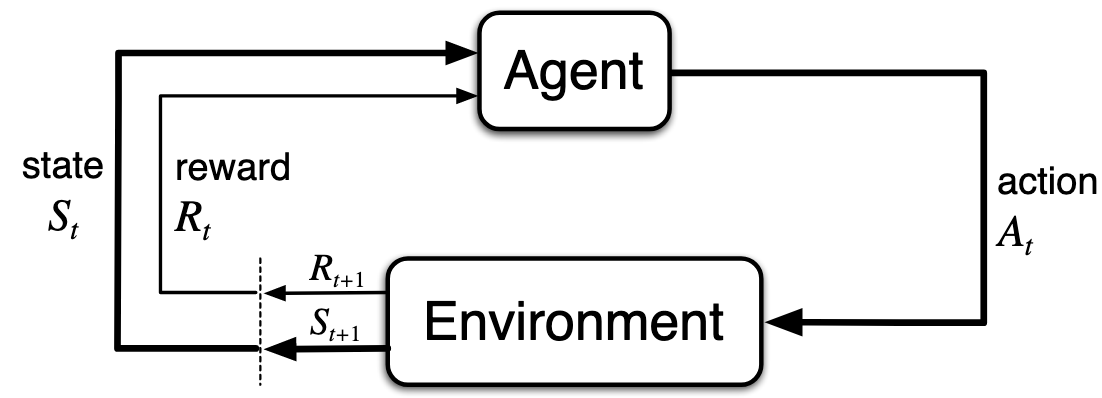
\includegraphics[scale=0.4]{images/agent_environment.png}
\end{figure}
\slidenote{joke: spend a lot of time here}
\slidenote{Neuroscience: human brain is believed to be devoted to the dopamine system reflects the reinforcement learning loop}
\slidenote{Phycology: Classical conditioning: how and why animals behaviour happens when you give them a treat}
\end{frame}

\begin{frame}{Motivation}
\begin{figure}
	\centering
	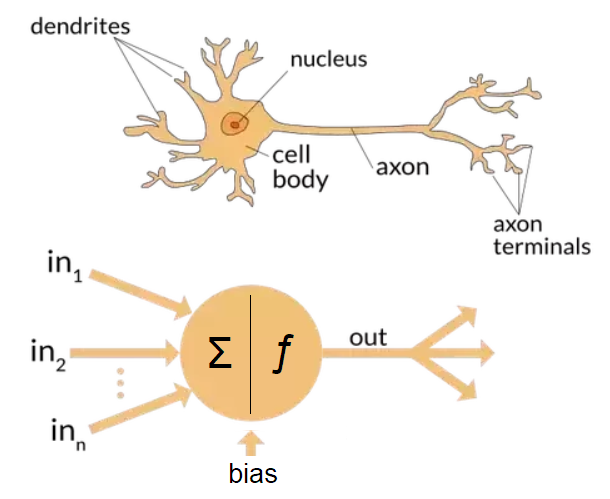
\includegraphics[scale=0.4]{images/neural_networks.png}
\end{figure}
\slidenote{Neural networks structured on how our brain performs computations with neurons}
\slidenote{Varying degrees of biological plausibility, but the point is that it was motivated by the human experience}
\end{frame}

\begin{frame}{Motivation}
\begin{itemize}
	\item Non-stationarity
	\item Credit Assignment
	\item Scaling
\end{itemize}
\slidenote{It is reasonable to then approach problems we see in multi-agent reinforcement learning too with the tools from human coordination/competition - communication}
\end{frame}


\section{Comm-MARL}
\begin{frame}{How do we communicate?}
\begin{figure}
	\centering
	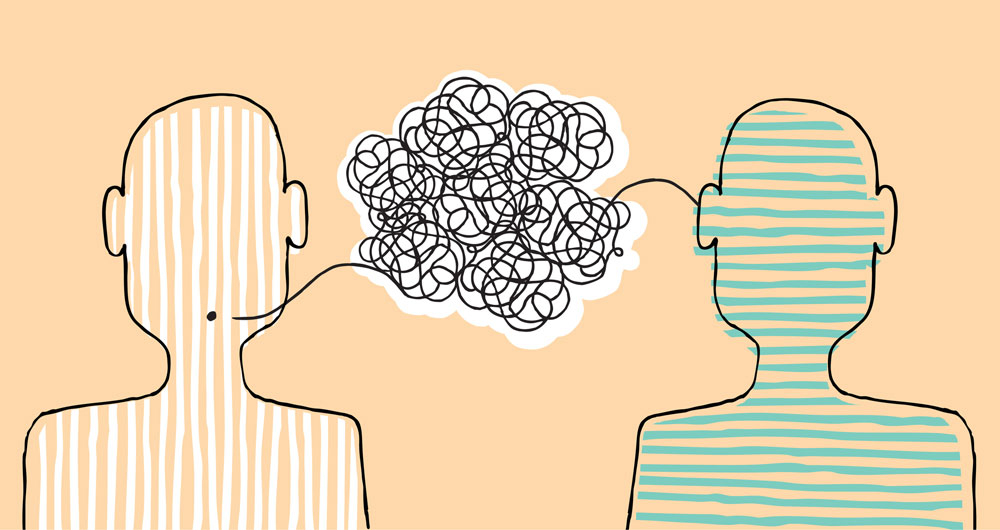
\includegraphics[scale=0.3]{images/communicate.jpg}
\end{figure}
\slidenote{Sign language, inflection}
\slidenote{finite lexicon with infinite utterances}	
\slidenote{Norm Chomsky}
\end{frame}

\begin{frame}{Dimensions of Comm-MARL}
    \scriptsize 
    \resizebox{\textwidth}{!}{
        \begin{tabular}{|>{\centering\arraybackslash}m{2.8cm}|>{\centering\arraybackslash}m{1cm}|>{\arraybackslash}m{5.5cm}|>{\centering\arraybackslash}m{2.8cm}|}
            \hline
            \textbf{Component} & \textbf{Index} & \textbf{Question} & \textbf{Dimension} \\
            \hline
            Problem Setting
            & 1 & What kind of behaviours are desired to emerge with communication? & Controlled Goals \\
            \cline{2-4}
            & 2 & How to fulfil realistic requirements? & Communication Constraints \\
            \cline{2-4}
            & 3 & Which type of agents to communicate with? & Communicatee Types \\
            \hline
            Communication Processes
            & 4 & When and how to build communication links among agents? & Communication policy \\
            \cline{2-4}
            & 5 & How to combine received messages? & Message combination \\
            \cline{2-4}
            & 6 & Which piece of information to share? & Communicated messages \\
            \cline{2-4}
            & 7 & How to integrate combined messages into learning models? & Inner integration \\
            \hline
            Training Processes 
            & 8 & How to train and improve communication? & Learning methods \\
            \cline{2-4}
            & 9 & How to utilise collected experience from agents? & Training schemes \\
            \hline
        \end{tabular}
    }
\end{frame}

\begin{frame}{Dimensions of Comm-MARL}
    \scriptsize 
    \resizebox{\textwidth}{!}{
        \begin{tabular}{|>{\centering\arraybackslash}m{2.8cm}|>{\centering\arraybackslash}m{1cm}|>{\arraybackslash}m{5.5cm}|>{\centering\arraybackslash}m{2.8cm}|}
            \hline
            \textbf{Component} & \textbf{Index} & \textbf{Question} & \textbf{Dimension} \\
            \hline
            Problem Setting
            & 1 & What kind of behaviours are desired to emerge with communication? & Controlled Goals \\
            \cline{2-4}
            & 2 & How to fulfil realistic requirements? & Communication Constraints \\
            \cline{2-4}
            & 3 & Which type of agents to communicate with? & \textcolor{red}{Communicatee Types} \\
            \hline
            Communication Processes
            & 4 & When and how to build communication links among agents? & Communication policy \\
            \cline{2-4}
            & 5 & How to combine received messages? & Message combination \\
            \cline{2-4}
            & 6 & Which piece of information to share? & Communicated messages \\
            \cline{2-4}
            & 7 & How to integrate combined messages into learning models? & Inner integration \\
            \hline
            Training Processes 
            & 8 & How to train and improve communication? & \textcolor{red}{Learning methods} \\
            \cline{2-4}
            & 9 & How to utilise collected experience from agents? & \textcolor{red}{Training schemes} \\
            \hline
        \end{tabular}
    }
\end{frame}

\begin{frame}{Method}
	\begin{enumerate}
		\item RIAL and DIAL \citep{foerster2016learning}
		\item CommNet \citep{sukhbaatar2016commnet}
		\item BiCNet \citep{peng2017bicnet}
		\item IC3Net \citep{singh2018ic3net}
		\item NeurComm \citep{chu2020NeurComm}
		\item HAMMER \citep{gupta2022HAMMER}
	\end{enumerate}
\slidenote{Differentiable and Reinforced Inter Agent Learning: Messages are output as part of a neural network}
\slidenote{Communication Network: Messages are not explicitly output but rather average of the states of the neural network}
\slidenote{Bidirectionally-Coordinated Networks: Bidirectional RNN hidden states passes forward then backward}
\slidenote{Individualized Controlled Continuous Communication Network: CommNet with a gating mechanism}
\slidenote{Neural communication protocol: Networked model where messages are the unions of observations, policy fingerprint, hidden state}
\slidenote{Heterogeneous Agents Mastering Messaging to Enhance Reinforcement learning: PPO with a central communicator called a proxy}
\end{frame}

\begin{frame}{Commuicateee Types}
\begin{figure}
	\centering
	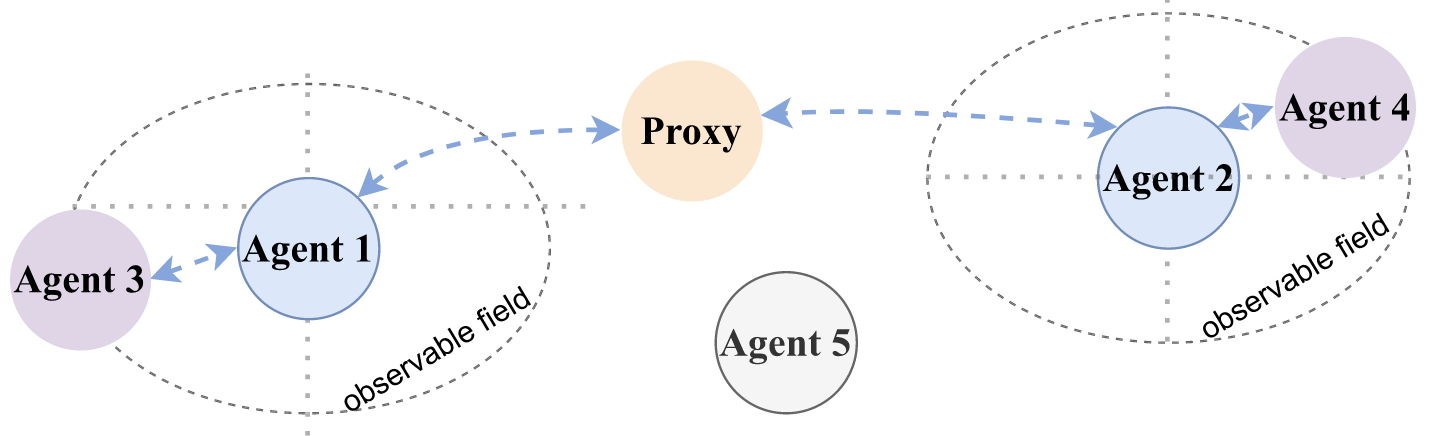
\includegraphics[scale=0.4]{images/communicatee.png}
\end{figure}
\slidenote{Nearby: Neurcomm create a network of agents connected}
\slidenote{IC3Net: Gating mechanism to communicate or not with other agents - competitive and mixed scenarios}
\slidenote{Proxy: Hammer - differentiable and reinforced}
\end{frame}

\begin{frame}{Learning Methods}
\begin{figure}
	\centering
	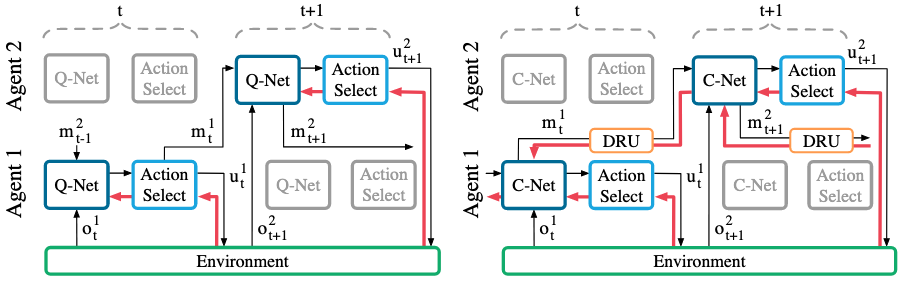
\includegraphics[scale=0.35]{images/rial_dial}
	\caption{\textbf{Left}: RIAL - \textbf{Right:} DIAL }
\end{figure}
\slidenote{RIAL and HAMMERv1: Reinforced}
\slidenote{FIAL and HAMMERv2,3: Differentiable}
\end{frame}

\begin{frame}{Training Schemes}
\begin{figure}
	\centering
	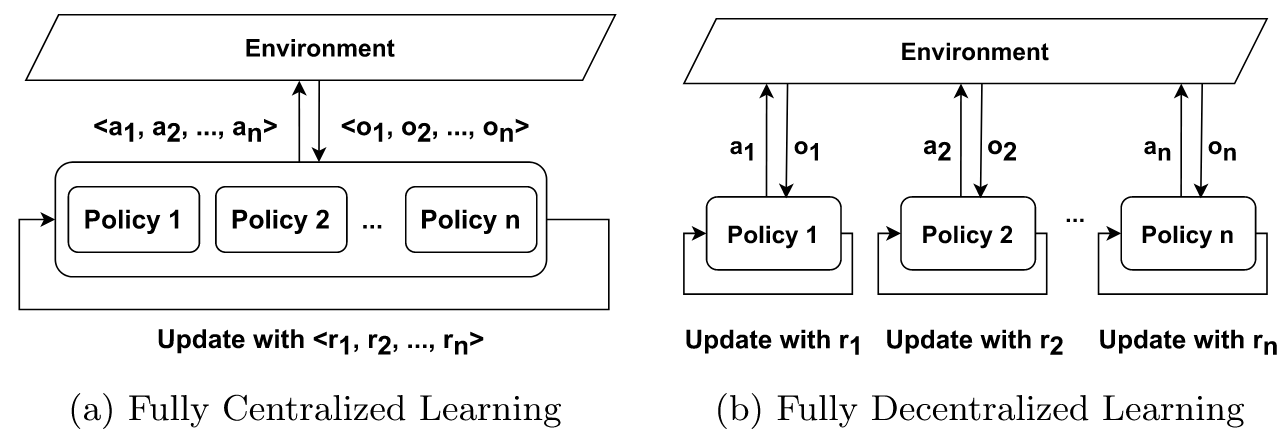
\includegraphics[scale=0.4]{images/training_schemes.png}
\end{figure}
\slidenote{Fully Centralised Learning: None}
\slidenote{Fully Decentralised Learning: NeurComm}
\end{frame}

\begin{frame}{Training Schemes}
\begin{figure}
	\centering
	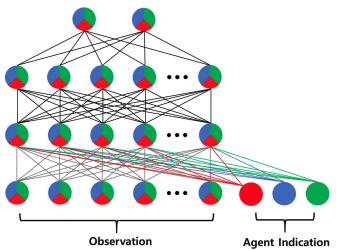
\includegraphics[scale=0.5]{images/parameter_sharing.png}
\end{figure}	
\slidenote{Everything: DIAL and RIAL, CommNet, IC3Net}
\end{frame}



\section{Investigation of Parameter Sharing}

\begin{frame}{NPS vs PS Model}
	\begin{figure}
		\centering
		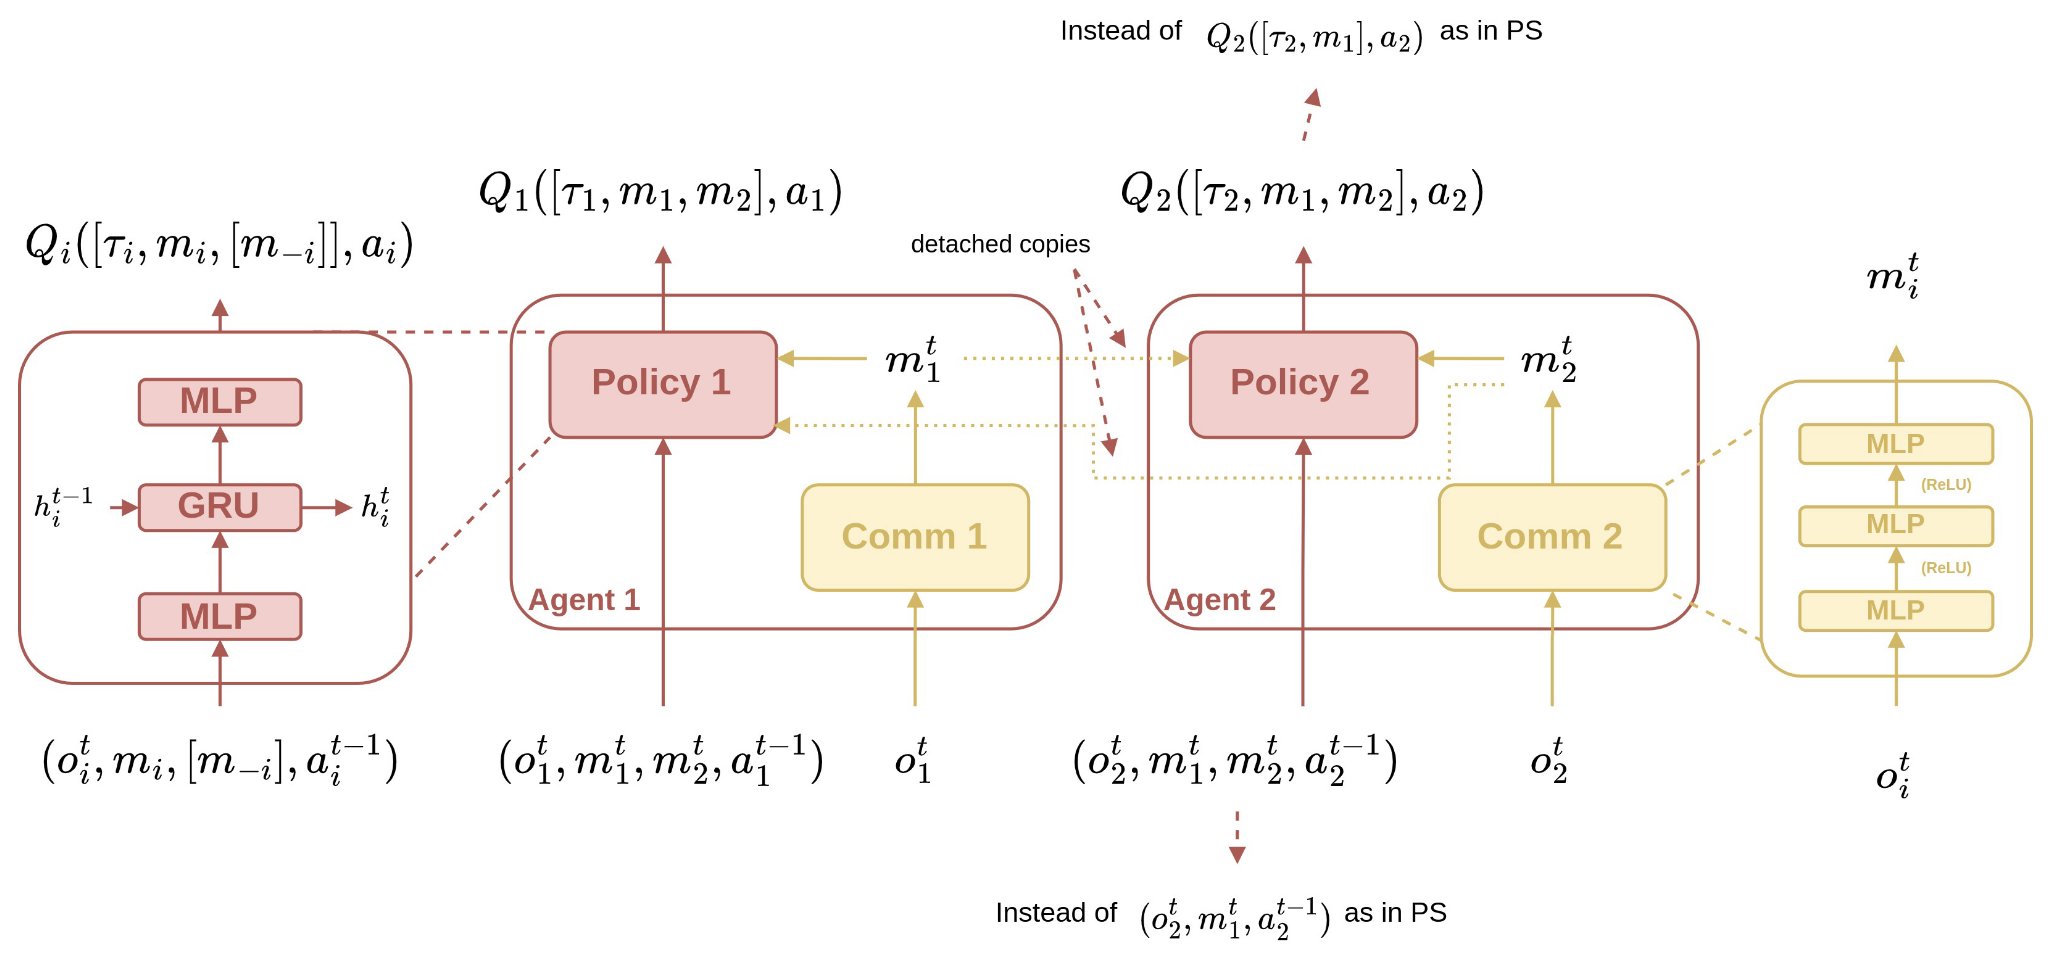
\includegraphics[scale=0.25]{images/nps_comm.png}
	\end{figure}
\slidenote{Detachment of the computational graph when not using parameter sharing - so they require their own message as input to keep the computational graph connected}
\slidenote{Formally show how the gradients will be calculated in this independent scheme}
\end{frame}

\begin{frame}{Results}
\end{frame}


\begin{frame}{References}
\tiny
\nocite{zhu2024survey}
\nocite{pina2024fully}
\bibliography{references}
\end{frame}

\end{document}